\documentclass[a4paper,fleqn]{cas-sc}

\usepackage[numbers,sort&compress]{natbib}
\usepackage{graphicx}
\usepackage{booktabs}

\begin{document}

\shorttitle{Short Article Title}
\shortauthors{First Author et al.}

\title[mode=title]{Research Article Title}

\author[1]{First Author}[orcid=0000-0000-0000-0000]
\ead{author@example.com}
\address[1]{organization={Institution Name},
             city={City},
             country={Country}}

\begin{abstract}
Replace this placeholder with an evidence-grounded abstract after the experiments and conclusions are stable.
\end{abstract}

\begin{keywords}
artificial intelligence \sep machine learning \sep reproducible research
\end{keywords}

\maketitle

\section{Introduction}
\label{sec:introduction}

Continuous structural health monitoring (SHM) provides a means of tracking the condition of bridges between scheduled inspections, but converting multichannel vibration measurements into reliable damage decisions remains difficult. Damage records are scarce, the response of an undamaged structure varies with excitation and environmental conditions, and the sensing system itself is not perfectly reliable. These constraints favor unsupervised or one-class formulations in which a model learns a reference representation from healthy data and subsequently flags departures from that representation. Full-scale bridge monitoring data illustrate both the value and the difficulty of this setting. Controlled progressive-damage campaigns provide measured structural changes, while long-term observations show that environmental variation can produce changes in modal properties comparable to those associated with damage \cite{peeters2001z24,maeck2003description,maeck2003damage}. A deployable detector must therefore remain sensitive to previously unseen damage without interpreting every change in the measurement process as a structural event.

Recent studies have advanced healthy-reference damage detection from several directions. Bayane et al. separated bridge measurements into comparable loading events, constructed statistical, time-frequency, and wavelet feature matrices, and compared five unsupervised detectors on a railway bridge that experienced brittle cracking \cite{bayane2024unsupervised}. Mousavi et al. combined raw acceleration with time-, frequency-, and wavelet-domain features in a multi-domain fusion autoencoder and evaluated the resulting digital-twin framework on two bridges \cite{mousavi2026digital}. Liu and Di integrated graph attention, recurrent temporal modeling, variational reconstruction, and deep support vector data description to learn a compact normal region from multichannel bridge data \cite{liu2026stvr}. These methods strengthen feature learning or normal-class modeling, but their principal experimental question is anomaly separation when the expected sensing configuration is available. They do not directly establish how a detector trained with a complete array behaves when different subsets of channels become unavailable during deployment.

This distinction is important because incomplete observation is not equivalent to ordinary signal noise. Communication interruption, sensor aging, power loss, and maintenance can remove an entire channel for a sustained interval. Replacing a missing channel with a constant changes the joint input distribution, while discarding it changes the dimensionality and invalidates a detector trained for a fixed sensor array. More importantly, loss of a structurally informative channel can reduce the separation between healthy and damaged responses even when the remaining measurements are internally consistent. Kullaa formalized the closely related diagnostic ambiguity among sensor faults, structural damage, and environmental or operational effects \cite{kullaa2011distinguishing}. The practical issue addressed here is narrower: given a healthy-only detector and a fixed array during training, can its damage sensitivity be retained when a random subset of sensors is absent at inference time?

Existing missing-data research provides useful components but does not fully answer this question. Entezami et al. developed an unsupervised meta-learning procedure for long-term modal data containing missing samples and severe environmental variation; missing observations are cleaned before segmented, locally robust anomaly analysis \cite{entezami2023meta}. Xin et al. fused time-, space-, and frequency-domain information to reconstruct continuous gaps in multichannel monitoring data, optimizing recovery fidelity on experimental and in-service bridge measurements \cite{xin2025recovery}. Wang et al. modeled inter-period and intra-period correlations to diagnose anomalous bridge-monitoring data and reduce false alarms associated with data-quality events \cite{wang2025online}. These studies address missing-value cleaning, signal recovery, or abnormal-data diagnosis. Accurate signal reconstruction, however, does not guarantee preservation of a downstream anomaly score. A recovery network optimized only for pointwise fidelity may map an unfamiliar damaged response toward the healthy manifold, which can make the reconstructed signal appear plausible while weakening damage evidence.

Sensor-placement research addresses a complementary problem. Shi et al. proposed a noise-assisted attention network for data-driven, unsupervised sensor-placement optimization and showed that damage could remain detectable after removing sensors selected as redundant \cite{shi2024sensor}. Optimal placement assumes that the retained subset is determined before monitoring or adapted under a defined optimization criterion. Unplanned sensor loss instead produces multiple observation masks after deployment, including subsets that were not selected for diagnostic sufficiency. Consequently, robustness to a designed sparse array cannot be treated as evidence of robustness to arbitrary missing channels. The latter requires a model that conditions explicitly on sensor availability and is trained across a distribution of masks.

Decision calibration creates a second failure mode. Even when missing-channel adaptation improves score ranking, a threshold estimated from complete observations may transfer poorly because the score distribution shifts with sensor availability. Alarm-processing approaches reduce false positives by using repeated exceedances or operating-condition-specific thresholds. Kamali et al., for example, used a binomial distribution classifier to convert repeated damage-index exceedances into alert and alarm states while preserving probability of detection \cite{kamali2024reducing}. Such decision logic operates after a damage index has been produced. It does not repair the representation shift induced by absent sensors, and a robust representation alone does not ensure a stable operating point. Representation adaptation and threshold behavior must therefore be evaluated separately through threshold-free ranking metrics and recall at a controlled false-positive rate.

The literature consequently leaves a specific gap between three established research streams: healthy-only damage detection, multichannel missing-data recovery, and sensor selection. Few studies formulate missing-sensor robustness as preservation of a pre-existing detector's representation and anomaly score, using only healthy data for adaptation and withholding test damage labels from architecture, score orientation, and threshold selection. Evidence is also limited on whether an improvement persists across independent training seeds and multiple nested sensor masks rather than one favorable corruption realization. This gap does not imply that missing-data recovery, mask-aware learning, or adaptive calibration is individually new. The unresolved question is whether these elements can be organized into a leakage-controlled protocol that preserves unseen-damage evidence as the available sensor set contracts.

To investigate this question, counteractive learning for missing measurements network (CLMM-Net), a mask-conditioned adapter built around a frozen healthy-only USAD detector. The source detector first learns complete healthy windows. A cross-sensor adapter then receives both the masked response and its availability mask and reconstructs only the unavailable channels. Training uses healthy windows with a hard-mask curriculum that includes random and sensor-importance-guided subsets. In addition to reconstruction error, the adapter is constrained to preserve the frozen detector's latent representation and anomaly score between complete and masked versions of the same healthy window. This objective differs from generic imputation because the recovered signal is optimized for compatibility with the downstream detector rather than waveform fidelity alone. Damage samples are not used to fit the detector or adapter.

The study adopts a severity-controlled protocol to evaluate damage detection under progressively increasing sensor loss. Raw multichannel acceleration records are partitioned at record level into training, validation, and test cohorts to prevent overlap between windows derived from the same record. Models are trained on healthy data, and random sensor masks are applied after preprocessing at increasing missing rates. The same nested masks are shared by CLMM and all baselines. Evaluation reports area under the receiver operating characteristic curve, average precision, balanced accuracy, recall, false-positive rate, precision, and F1 score. Neural methods are repeated over ten independent seeds, while multiple masks are averaged within each seed before between-seed variability is calculated. Random sensor loss is the primary claim; targeted removal of the most informative sensors is retained as a stress test rather than assumed to be recoverable.

The contributions of this work are as follows:
\begin{enumerate}
	\item Missing-sensor bridge SHM is formulated as detector-preserving, healthy-only adaptation. This formulation separates structural anomaly evidence from data-completion accuracy and excludes damage samples from detector and adapter training.
	
	\item CLMM integrates an explicit availability mask, cross-sensor reconstruction, hard-mask curriculum learning, and latent- and score-consistency constraints with a frozen USAD detector. The contribution of each component is assessed through controlled ablation experiments.
	
	\item A reproducible evaluation protocol is established using record-level splits, common nested masks, fixed metric definitions, ten neural-network seeds, and paired comparisons with PCA-SPE, LSTM-AE, USAD, TranAD, TimesNet, ModernTCN, and ScatterAD. The protocol distinguishes ranking robustness from threshold transfer and explicitly reports performance limitations under targeted sensor loss.
\end{enumerate}

\section{Related work}
\label{sec:related}
\subsection{Unsupervised damage detection in structural health monitoring}
\label{subsec:unsupervised-shm}

Data-driven structural health monitoring (SHM) methods commonly rely on supervised or unsupervised learning. Although supervised models can directly distinguish predefined structural conditions, their practical application is limited by the scarcity of measured damage data. Structural damage is infrequent, potentially unsafe to reproduce, and dependent on damage location, severity, structural configuration, excitation, and environmental conditions. Unsupervised and one-class methods address this limitation by learning the distribution of healthy structural responses and identifying observations that deviate from the established reference condition. These methods include statistical distance measures, clustering, density estimation, one-class classification, isolation-based detection, and reconstruction-based deep learning.

Existing studies have investigated several approaches to improve healthy-only damage detection. Bayane et al. combined statistical, time--frequency, and wavelet features with multiple unsupervised anomaly detectors for real-time bridge monitoring \cite{bayane2024unsupervised}. Their approach emphasizes the importance of separating measurements into comparable loading events before anomaly analysis. Reconstruction-based methods instead learn nonlinear representations directly from monitoring signals. Mousavi et al. developed a multi-domain fusion autoencoder that integrates raw acceleration measurements with time-, frequency-, and wavelet-domain features \cite{mousavi2026digital}. This formulation exploits complementary information from multiple signal representations rather than relying on a single damage indicator. Liu and Di combined graph attention, recurrent temporal modeling, variational reconstruction, and deep support vector data description to model spatial dependencies, temporal evolution, and the boundary of the healthy condition \cite{liu2026stvr}. Collectively, these studies show that unsupervised detection can benefit from event conditioning, multi-domain feature fusion, and joint spatio-temporal representation learning.

Despite these advances, unsupervised SHM detectors are generally developed under a predefined sensing configuration. Their input dimensions, cross-sensor relationships, latent representations, anomaly-score distributions, and decision thresholds are therefore associated with a particular set of available channels. When one or more sensors become unavailable, constant-value replacement may introduce an artificial distribution shift, while direct channel removal changes the expected model input. The resulting anomaly-score variation may reflect incomplete observation rather than a change in structural condition. Moreover, the loss of structurally informative channels can reduce the separability between healthy and damaged responses. Consequently, performance obtained under complete observations does not establish detector reliability under changing sensor availability. This limitation motivates a separate examination of missing data in multichannel structural monitoring and of learning strategies designed for incomplete sensor observations.

\subsection{Missing sensor measurements in vibration-based structural health monitoring}

Prior studies address missing measurements at different stages of structural health monitoring. At the feature level, Entezami et al.\ \cite{entezami2023meta} screened incomplete modal observations before applying unsupervised anomaly detection under varying environmental conditions. At the signal level, Xin et al.\ \cite{xin2025recovery} combined multichannel decomposition with physics-aided temporal convolution to recover contiguous gaps in monitoring signals. The former study used data screening to prepare modal features for anomaly detection, whereas the latter evaluated how accurately missing signals could be reconstructed.

Sensor placement research examines how the choice of channels affects damage detection. Shi et al.\ \cite{shi2024sensor} used a noise-assisted attention network to identify sensor locations suited to unsupervised damage detection. In that setting, the retained channels were selected for their diagnostic value. When sensor loss occurs during monitoring, the available subset is determined by which channels remain operational. The performance of a deliberately selected sensor array therefore provides limited evidence about how an existing detector responds to unplanned channel loss.

The studies reviewed above leave open a specific question about damage detection under incomplete observations. Detection after screening incomplete modal samples does not quantify the effect of losing an entire vibration channel during an analysis window. Likewise, signal recovery error does not quantify how an existing detector's anomaly scores change after reconstruction. Two aspects of detector performance are relevant in this setting. The first is whether damaged responses remain distinguishable from healthy responses in the score ranking. The second is whether a threshold calibrated on complete measurements still provides an acceptable balance between damage recall and false alarms when the available sensor subset changes.
\subsection{Learning from incomplete multivariate time series}
\label{subsec:incomplete-mts}

Methods for incomplete multivariate time series differ in how they connect missing-data recovery to downstream detection. Du et al.\ \cite{du2023saits} developed SAITS, which uses self-attention to estimate missing values from temporal and cross-variable dependencies. Its training objective combines reconstruction of observed entries with prediction of artificially masked entries. This masking strategy provides a way to train imputation models on available measurements, although the ability to recover isolated missing entries gives limited evidence about a setting in which an entire channel is absent throughout an analysis window.

Other methods incorporate missingness directly into anomaly detection. Yang et al.\ \cite{yang2023probabilistic} used expectation maximization to couple missing-value estimation with unsupervised density estimation in a probabilistic graphical model. Zheng et al.\ \cite{zheng2024gstpro} modeled irregular multivariate observations with a graph spatiotemporal process and derived anomaly scores from its predictive distributions. These approaches integrate incomplete observations into the learning or scoring of the detector itself.

A different evaluation question arises when a detector has already been fitted on complete healthy measurements and its parameters are held fixed. Under whole-channel loss, the relevant outcome is whether the available measurements and any recovered signals retain the information used by that detector. The methods reviewed above motivate evaluating imputation through downstream detection performance, with separate attention to anomaly-score ranking and alarm performance at the original decision threshold.

\section{Methodology}
\label{sec:methods}

% Describe the proposed method with enough precision to reproduce it.
% Follow the equation guidance when introducing mathematical notation.

\section{Experimental setup}
\label{sec:experimental-setup}

% Record datasets, splits, preprocessing, baselines, metrics, seeds, hardware,
% implementation details, and statistical protocol from experiment evidence.

\section{Results and discussion}
\label{sec:results-discussion}

\subsection{Baseline performance under random sensor loss}
\label{subsec:baseline-sensor-loss}

On Z24, the mean record-level ROC-AUC decreased from complete observations through each successive sensor-loss level for all six baselines shown in Fig.~\ref{fig:z24-baseline-sensor-loss}. USAD maintained the highest mean ROC-AUC across the evaluated conditions, although its value declined from 0.9106 with complete observations to 0.7867 at 30\% sensor loss.

\begin{figure}[pos=!htbp]
  \centering
  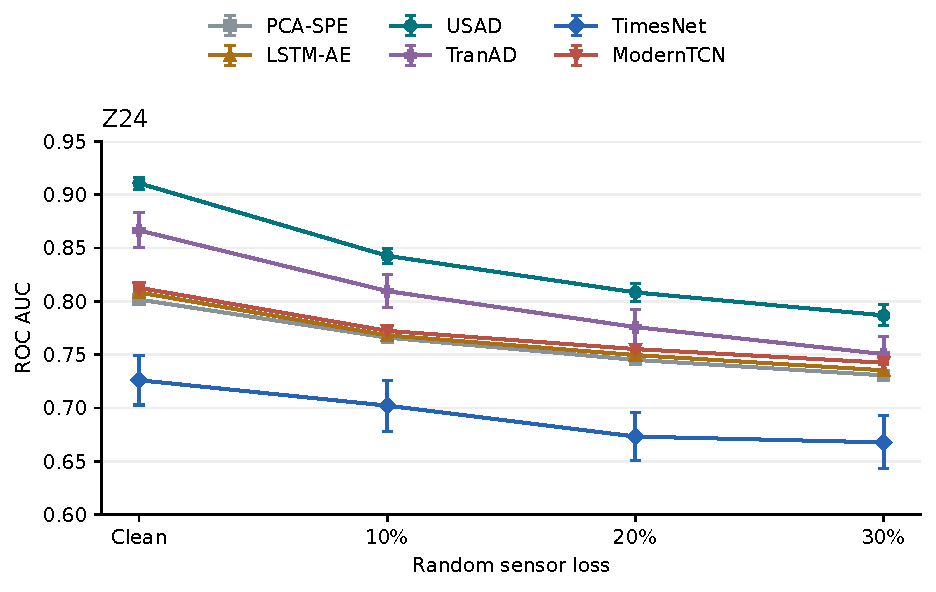
\includegraphics[width=0.88\linewidth]{figs/z24_baseline_roc_auc.pdf}
  \caption{Record-level ROC-AUC of Z24 baselines from complete observations to 30\% random sensor loss. For neural baselines, five masks were averaged within each seed at each nonzero loss rate, and the plots show the mean and standard deviation across ten seeds. PCA-SPE used one deterministic fit. ScatterAD was unavailable for this Z24 sweep.}
  \label{fig:z24-baseline-sensor-loss}
\end{figure}

On HellBridge, the mean window-level recall, balanced accuracy, and F1 score decreased at each successive sensor-loss level for all seven baselines (Fig.~\ref{fig:hellbridge-baseline-sensor-loss}). For example, USAD recall decreased from 0.2081 to 0.0699 at 30\% sensor loss under the threshold calibrated on complete healthy measurements. The Z24 result quantifies a loss in ranking performance, while the HellBridge result quantifies a loss in detection performance at a fixed operating threshold.

\begin{figure}[pos=!htbp]
  \centering
  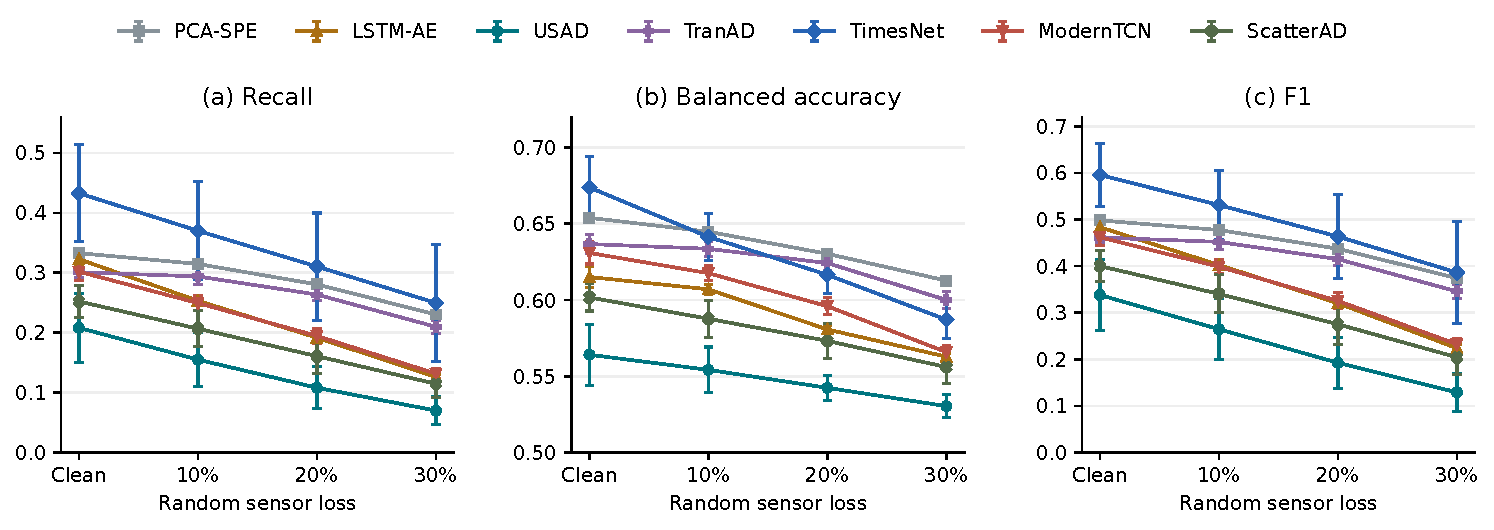
\includegraphics[width=\linewidth]{figs/hellbridge_baseline_sensor_loss.pdf}
  \caption{Window-level (a) recall, (b) balanced accuracy, and (c) F1 score on HellBridge under increasing random sensor loss. The threshold for each fitted model was calibrated on complete healthy measurements and held fixed across sensor-loss conditions. For neural baselines, error bars show the standard deviation across ten seeds after averaging five masks within each seed at each nonzero loss rate. PCA-SPE used one deterministic fit.}
  \label{fig:hellbridge-baseline-sensor-loss}
\end{figure}

% Flush the Results figures before the Conclusion and bibliography.
\clearpage
\section{Conclusion}
\label{sec:conclusion}

% Answer the research question without introducing unsupported new claims.

\section*{Declaration of competing interest}
The authors declare that they have no known competing financial interests or personal relationships that could have appeared to influence the work reported in this paper.

\section*{Data availability}
Replace this placeholder with the actual data and code availability statement.

\bibliographystyle{model1-num-names}
\bibliography{references}

\end{document}
